%%%%%%%%%%%%%%%%%%%%%%%%%%%%%%%%%%%%%%%%%%%%%%%%%%%%%%%%%%%%%%%%%%%%%%%%%%%%%%%%%%%%%%%%%%%%%%%%%%%
%%%%%%%%%%%%%%%%%%%%%%%%%%%%%%%%%%%%%%%%%%%%%%%%%%%%%%%%%%%%%%%%%%%%%%%%%%%%%%%%%%%%%%%%%%%%%%%%%%%
\chapter{Resultados}

En cada canal que conforma el PSG (EEG, EOG y EMG), 
cada una de las \'epocas consideradas fue clasificada como 
''\'Epoca Posiblemente Estacionaria'' (EPE) si no pudo ser rechazado la hip\'otesis de 
estacionariedad usando el test PSR ($\alpha = 0.05$), mientra que 
%el rechazo de esta misma 
%hip\'otesis es argumento ''suficiente'' para afirmar que el segmento de registro en cuenti\'on
%puede ser clasificado omo no.estacionario.
fue clasificado como ''No-estacionario'' en caso contrario. Variar el valor cr\'itico
para la clasificaci\'on no pareci\'o generar diferencias significativas.

La cantidad de \'epocas que no fueron para las cuales no es posible rechazar la hip\'otesis de
estacionariedad ($\alpha=0.05$)
clasificadas como ''Posiblemente Estacionarias'' (PE). 
La cantidad de \'epocas PE en cada individuo %con respecto a la cantidad total de \'epocas
durante el sue\~no MOR y no-MOR
muestra en las tablas \ref{total_gpos_mor}, \ref{total_gpos_nmor} y
\ref{total_gpos_total}; debido a que entre los sujetos hubo una gran variabilidad entre el tiempo 
que permanecieron en sue\~no MOR, se sugiri\'o comparar no el total de \'epocas PE sino
la proporci\'on --con respecto a la duraci\'on, medida en \'epocas-- de estas etapas, 
mustr\'andose estos resultados en las tablas \ref{gpos_mor}, \ref{gpos_nmor} y
\ref{gpos_total}. En estas \'ultimas tablas, se han calculado promedios y desviaciones
est\'andar muestrales entre los dos grupos que son comparados.


\begin{SidewaysFigure}
\centering
\begin{tabular}{c||ccccc||cccc||ccc}
&VCR&MJH&JAE&GHA&MFGR&CLO&RLO&RRU&JGZ&FGH&MGG&EMT \\
\hline
C3& & &*& &***& &**&*& & & &  \\
C4& & &***& &***& &***& & & &*&  \\
CZ& & & & &***& & & & & &***&  \\
F3& & & &***& & &***& & & &*&  \\
F4& & & &***& & &***& & & &***&  \\
F7& & &***& &*& & &***& & &***&  \\
F8& & & &***&*& &*&***& & &***&  \\
FP1&*& & &***& & & &***& & &***&  \\
FP2& & & &***&*& & &**& & &***&  \\
FZ& & & &***& & &***&*& & &*&  \\
O1&***& & &***& & & &*& &*& &  \\
O2&*& &*&***& & &***& & & &***&  \\
P3& & &*&*&***& &**& & & &*&  \\
P4& & &***&*&***& & & & &*&***&  \\
PZ& & &***& &***& & & & & &***&  \\
T3&***& &**& &***& &***& & & & &  \\
T4& & & &*&*& &***& & & &*&* \\
T5&*& & &***& & &***& & & & &  \\
T6& & &*&*&*& & & & & &***&  \\
LOG&***& &***&***&**&***&**&***&*& &***&  \\
ROG&***& &***&***&*&*&***&*&*& &***&  \\
EMG& & & & & &***& &*& & & & 
\end{tabular}
\caption{Diferencias significativas para la comparaci\'on entre la proporci\'on
de \'epocas PE en sue\~no MOR (fase R) y no-MOR (fases W y N).
Los asteriscos representan el pvalor con el cual se rechaza la hip\'otesis de
que las diferencias son significativas: *=0.05 , **=0.01 , ***=0.005}
\label{comparacion_mor_vs_total}
\end{SidewaysFigure}

Como un primer an\'alisis, para cada sujeto y en cada canal 
se compar\'o la proporci\'on de \'epocas PE en sue\~no MOR contra el registro completo;
el fin de ello es verificar si el sue\~no MOR --entendido como muestra no-aleatoria
del sue\~no-- tiene propiedades similares o no, y si \'esta similaridad pudiera estar
relacionada con el PDC del paciente. 
Las comparaciones se llevaron a cabo usando una prueba $\chi^{2}$ para proporciones,
y los resultados se muestran en la tabla \ref{comparacion_mor_vs_total}.
Se encontr\'o que no hay una relaci\'on clara entre el estado de salud del sujeto y
la aparici\'on de diferencias significativas entre estas proporciones; en la secci\'on
de discusi\'on se mencionan algunos datos que se ''recuperaron'' de este an\'alisis.

Posteriormente se procedi\'o a comparar, por cada canal, si la proporci\'on de \'epocas PE
presenta diferencias significativas entre los grupos. Esta comparaci\'on se realiz\'o tomando
en cuenta las \'epocas de sue\~no MOR, de sue\~no no-MOR, y el registro completo 
--ver, respectivamente, tablas \ref{gpos_mor}, \ref{gpos_nmor}, \ref{gpos_total}.
Para una mejor visualizaci\'on de estos, se han graficado
% que representan
%las proporciones respectivas de cada sujeto --para ambos grupos.
en la figura \ref{comparacion_graf}
los datos de las tablas \ref{gpos_mor}, \ref{gpos_nmor} y
\ref{gpos_total}.

\begin{figure}
\centering
\subfloat[Comparaci\'on entre \'epocas MOR (fase R)]{
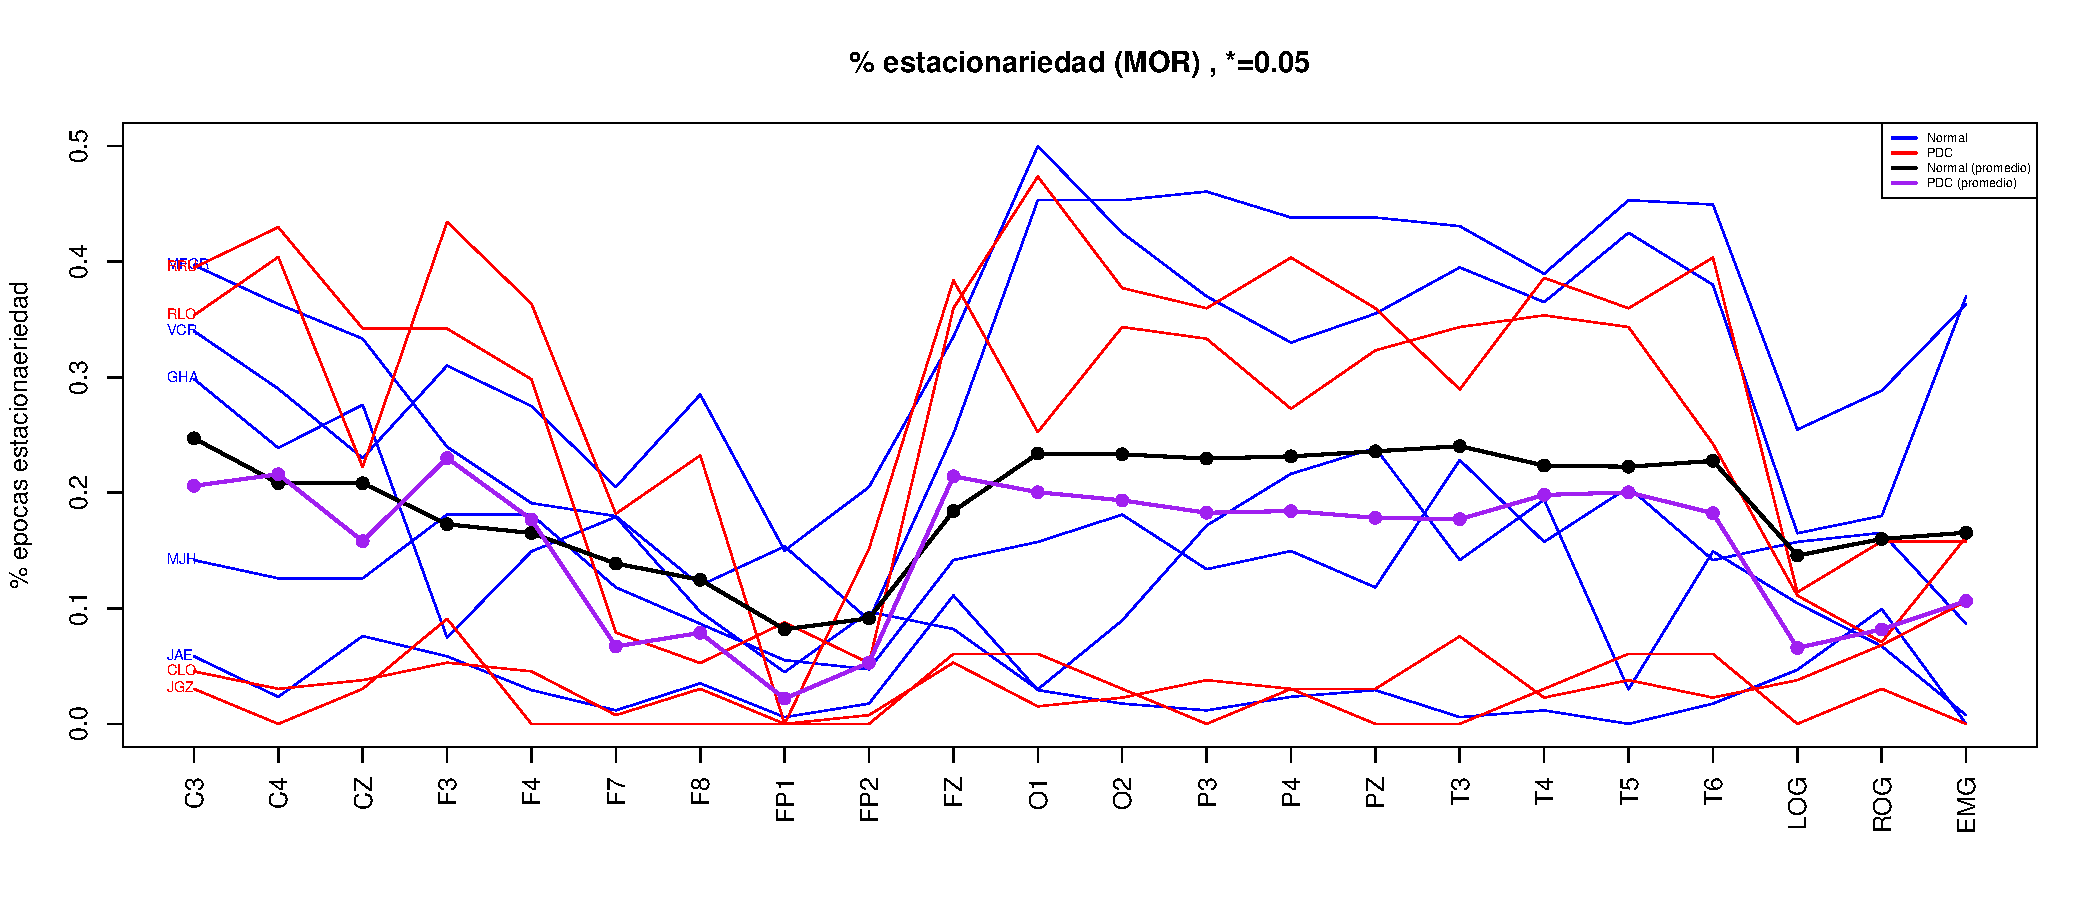
\includegraphics[width=0.9\linewidth]
{./material170331/Comparacion_gpos_MOR.pdf} 
}\\
\subfloat[Comparaci\'on entre \'epocas no-MOR (fases W y N)]{
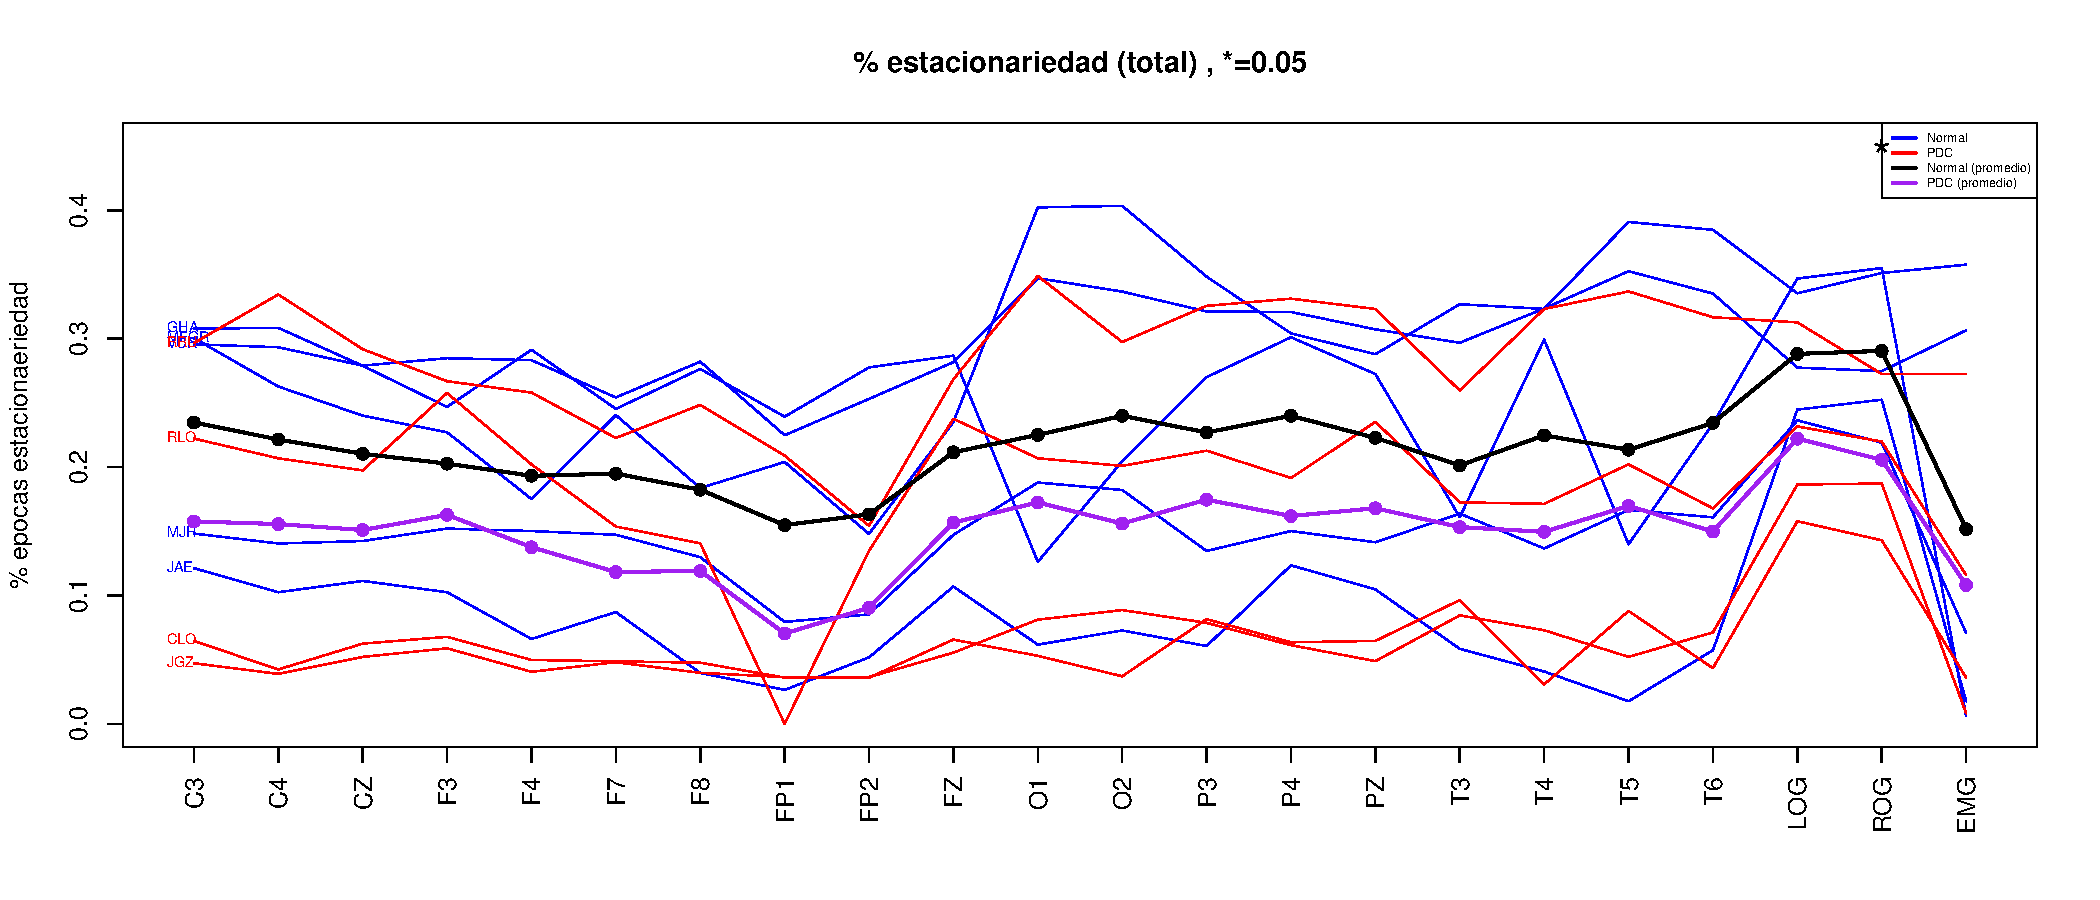
\includegraphics[width=0.9\linewidth]
{./material170331/Comparacion_gpos_NMOR.pdf} 
}\\
\subfloat[Comparaci\'on entre el total de \'epocas registradas]{
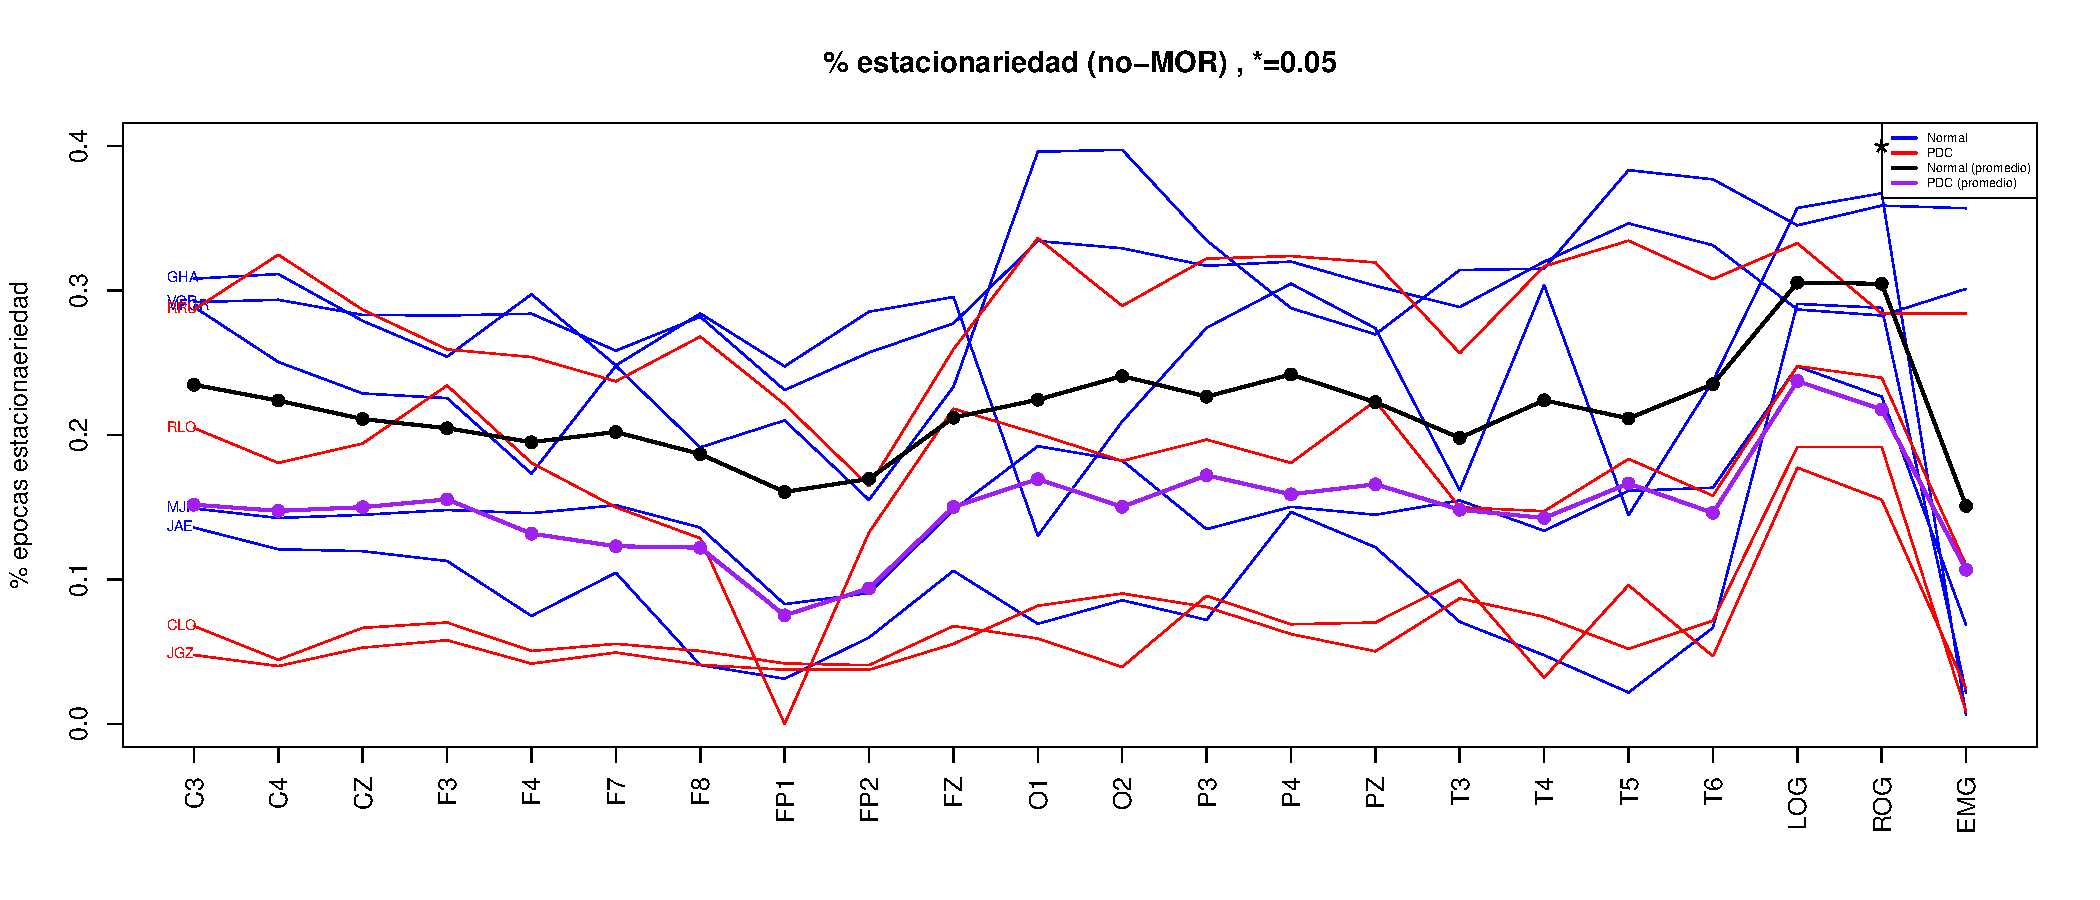
\includegraphics[width=0.9\linewidth]
{./material170331/Comparacion_gpos_TOT.pdf} 
}\\
\caption{Comparaci\'on entre las proporciones de \'epocas PE en diferentes
etapas de sue\~no; 
se sobrelapan en diferentes colores los sujetos con y sin PDC.}
\label{comparacion_graf}
\end{figure}

La comparaci\'on per se se llev\'o a cabo usando las pruebas %no param\'etrica
$t$ de Student y $U$ de Mann-Whitney-Wilcoxon.
El primer test arroja diferencias significativas para los canales LOG, ROG y EMG, mientras que
el segundo indica que no hay diferencias significativas. 

Debido a que los canales
donde se hallaron diferencias significativas no corresponden a registros de actividad
cerebral, se considera que \textbf{esta caracter\'istica no proporciona evidencias
suficientes sobre diferencias significativas entre adultos mayores con y sin PDC diagnosticado}.
Este resultado es clave en el desarrollo de este trabajo.

%%%%%%%%%%%%%%%%%%%%%%%%%%%%%%%%%%%%%%%%%%%%%%%%%%%%%%%%%%%%%%%%%%%%%%%%%%%%%%%%%%%%%%%%%%%%%%%%%%%
%%%%%%%%%%%%%%%%%%%%%%%%%%%%%%%%%%%%%%%%%%%%%%%%%%%%%%%%%%%%%%%%%%%%%%%%%%%%%%%%%%%%%%%%%%%%%%%%%%%